\documentclass[1p]{elsarticle_modified}
%\bibliographystyle{elsarticle-num}

%\usepackage[colorlinks]{hyperref}
%\usepackage{abbrmath_seonhwa} %\Abb, \Ascr, \Acal ,\Abf, \Afrak
\usepackage{amsfonts}
\usepackage{amssymb}
\usepackage{amsmath}
\usepackage{amsthm}
\usepackage{scalefnt}
\usepackage{amsbsy}
\usepackage{kotex}
\usepackage{caption}
\usepackage{subfig}
\usepackage{color}
\usepackage{graphicx}
\usepackage{xcolor} %% white, black, red, green, blue, cyan, magenta, yellow
\usepackage{float}
\usepackage{setspace}
\usepackage{hyperref}

\usepackage{tikz}
\usetikzlibrary{arrows}

\usepackage{multirow}
\usepackage{array} % fixed length table
\usepackage{hhline}

%%%%%%%%%%%%%%%%%%%%%
\makeatletter
\renewcommand*\env@matrix[1][\arraystretch]{%
	\edef\arraystretch{#1}%
	\hskip -\arraycolsep
	\let\@ifnextchar\new@ifnextchar
	\array{*\c@MaxMatrixCols c}}
\makeatother %https://tex.stackexchange.com/questions/14071/how-can-i-increase-the-line-spacing-in-a-matrix
%%%%%%%%%%%%%%%

\usepackage[normalem]{ulem}

\newcommand{\msout}[1]{\ifmmode\text{\sout{\ensuremath{#1}}}\else\sout{#1}\fi}
%SOURCE: \msout is \stkout macro in https://tex.stackexchange.com/questions/20609/strikeout-in-math-mode

\newcommand{\cancel}[1]{
	\ifmmode
	{\color{red}\msout{#1}}
	\else
	{\color{red}\sout{#1}}
	\fi
}

\newcommand{\add}[1]{
	{\color{blue}\uwave{#1}}
}

\newcommand{\replace}[2]{
	\ifmmode
	{\color{red}\msout{#1}}{\color{blue}\uwave{#2}}
	\else
	{\color{red}\sout{#1}}{\color{blue}\uwave{#2}}
	\fi
}

\newcommand{\Sol}{\mathcal{S}} %segment
\newcommand{\D}{D} %diagram
\newcommand{\A}{\mathcal{A}} %arc


%%%%%%%%%%%%%%%%%%%%%%%%%%%%%5 test

\def\sl{\operatorname{\textup{SL}}(2,\Cbb)}
\def\psl{\operatorname{\textup{PSL}}(2,\Cbb)}
\def\quan{\mkern 1mu \triangleright \mkern 1mu}

\theoremstyle{definition}
\newtheorem{thm}{Theorem}[section]
\newtheorem{prop}[thm]{Proposition}
\newtheorem{lem}[thm]{Lemma}
\newtheorem{ques}[thm]{Question}
\newtheorem{cor}[thm]{Corollary}
\newtheorem{defn}[thm]{Definition}
\newtheorem{exam}[thm]{Example}
\newtheorem{rmk}[thm]{Remark}
\newtheorem{alg}[thm]{Algorithm}

\newcommand{\I}{\sqrt{-1}}
\begin{document}

%\begin{frontmatter}
%
%\title{Boundary parabolic representations of knots up to 8 crossings}
%
%%% Group authors per affiliation:
%\author{Yunhi Cho} 
%\address{Department of Mathematics, University of Seoul, Seoul, Korea}
%\ead{yhcho@uos.ac.kr}
%
%
%\author{Seonhwa Kim} %\fnref{s_kim}}
%\address{Center for Geometry and Physics, Institute for Basic Science, Pohang, 37673, Korea}
%\ead{ryeona17@ibs.re.kr}
%
%\author{Hyuk Kim}
%\address{Department of Mathematical Sciences, Seoul National University, Seoul 08826, Korea}
%\ead{hyukkim@snu.ac.kr}
%
%\author{Seokbeom Yoon}
%\address{Department of Mathematical Sciences, Seoul National University, Seoul, 08826,  Korea}
%\ead{sbyoon15@snu.ac.kr}
%
%\begin{abstract}
%We find all boundary parabolic representation of knots up to 8 crossings.
%
%\end{abstract}
%\begin{keyword}
%    \MSC[2010] 57M25 
%\end{keyword}
%
%\end{frontmatter}

%\linenumbers
%\tableofcontents
%
\newcommand\colored[1]{\textcolor{white}{\rule[-0.35ex]{0.8em}{1.4ex}}\kern-0.8em\color{red} #1}%
%\newcommand\colored[1]{\textcolor{white}{ #1}\kern-2.17ex	\textcolor{white}{ #1}\kern-1.81ex	\textcolor{white}{ #1}\kern-2.15ex\color{red}#1	}

{\Large $\underline{12a_{0901}~(K12a_{0901})}$}

\setlength{\tabcolsep}{10pt}
\renewcommand{\arraystretch}{1.6}
\vspace{1cm}\begin{tabular}{m{100pt}>{\centering\arraybackslash}m{274pt}}
\multirow{5}{120pt}{
	\centering
	\includegraphics[width=112pt]{../../../GIT/diagram.site/Diagrams/png/1702_12a_0901.png}\\
\ \ \ A knot diagram\footnotemark}&
\allowdisplaybreaks
\textbf{Linearized knot diagam} \\
\cline{2-2}
 &
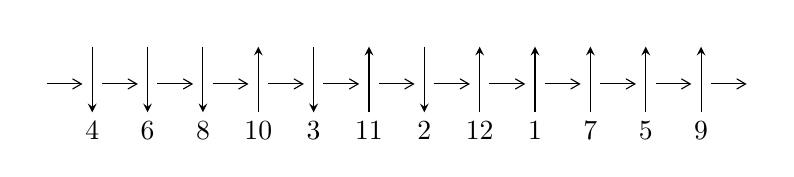
\begin{tikzpicture}[x=20pt, y=17pt]
	% nodes
	\node (C0) at (0, 0) {};
	\node (C1) at (1, 0) {};
	\node (C1U) at (1, +1) {};
	\node (C1D) at (1, -1) {4};

	\node (C2) at (2, 0) {};
	\node (C2U) at (2, +1) {};
	\node (C2D) at (2, -1) {6};

	\node (C3) at (3, 0) {};
	\node (C3U) at (3, +1) {};
	\node (C3D) at (3, -1) {8};

	\node (C4) at (4, 0) {};
	\node (C4U) at (4, +1) {};
	\node (C4D) at (4, -1) {10};

	\node (C5) at (5, 0) {};
	\node (C5U) at (5, +1) {};
	\node (C5D) at (5, -1) {3};

	\node (C6) at (6, 0) {};
	\node (C6U) at (6, +1) {};
	\node (C6D) at (6, -1) {11};

	\node (C7) at (7, 0) {};
	\node (C7U) at (7, +1) {};
	\node (C7D) at (7, -1) {2};

	\node (C8) at (8, 0) {};
	\node (C8U) at (8, +1) {};
	\node (C8D) at (8, -1) {12};

	\node (C9) at (9, 0) {};
	\node (C9U) at (9, +1) {};
	\node (C9D) at (9, -1) {1};

	\node (C10) at (10, 0) {};
	\node (C10U) at (10, +1) {};
	\node (C10D) at (10, -1) {7};

	\node (C11) at (11, 0) {};
	\node (C11U) at (11, +1) {};
	\node (C11D) at (11, -1) {5};

	\node (C12) at (12, 0) {};
	\node (C12U) at (12, +1) {};
	\node (C12D) at (12, -1) {9};
	\node (C13) at (13, 0) {};

	% arrows
	\draw[->,>={angle 60}]
	(C0) edge (C1) (C1) edge (C2) (C2) edge (C3) (C3) edge (C4) (C4) edge (C5) (C5) edge (C6) (C6) edge (C7) (C7) edge (C8) (C8) edge (C9) (C9) edge (C10) (C10) edge (C11) (C11) edge (C12) (C12) edge (C13) ;	\draw[->,>=stealth]
	(C1U) edge (C1D) (C2U) edge (C2D) (C3U) edge (C3D) (C4D) edge (C4U) (C5U) edge (C5D) (C6D) edge (C6U) (C7U) edge (C7D) (C8D) edge (C8U) (C9D) edge (C9U) (C10D) edge (C10U) (C11D) edge (C11U) (C12D) edge (C12U) ;
	\end{tikzpicture} \\
\hhline{~~} \\& 
\textbf{Solving Sequence} \\ \cline{2-2} 
 &
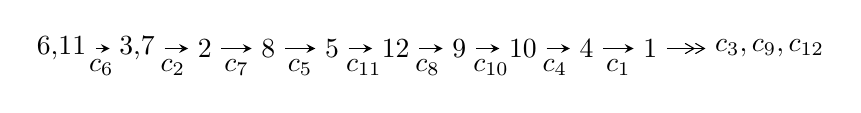
\begin{tikzpicture}[x=23pt, y=7pt]
	% node
	\node (A0) at (-1/8, 0) {6,11};
	\node (A1) at (17/16, 0) {3,7};
	\node (A2) at (17/8, 0) {2};
	\node (A3) at (25/8, 0) {8};
	\node (A4) at (33/8, 0) {5};
	\node (A5) at (41/8, 0) {12};
	\node (A6) at (49/8, 0) {9};
	\node (A7) at (57/8, 0) {10};
	\node (A8) at (65/8, 0) {4};
	\node (A9) at (73/8, 0) {1};
	\node (C1) at (1/2, -1) {$c_{6}$};
	\node (C2) at (13/8, -1) {$c_{2}$};
	\node (C3) at (21/8, -1) {$c_{7}$};
	\node (C4) at (29/8, -1) {$c_{5}$};
	\node (C5) at (37/8, -1) {$c_{11}$};
	\node (C6) at (45/8, -1) {$c_{8}$};
	\node (C7) at (53/8, -1) {$c_{10}$};
	\node (C8) at (61/8, -1) {$c_{4}$};
	\node (C9) at (69/8, -1) {$c_{1}$};
	\node (A10) at (11, 0) {$c_{3},c_{9},c_{12}$};

	% edge
	\draw[->,>=stealth]	
	(A0) edge (A1) (A1) edge (A2) (A2) edge (A3) (A3) edge (A4) (A4) edge (A5) (A5) edge (A6) (A6) edge (A7) (A7) edge (A8) (A8) edge (A9) ;
	\draw[->>,>={angle 60}]	
	(A9) edge (A10);
\end{tikzpicture} \\ 

\end{tabular} \\

\footnotetext{
The image of knot diagram is generated by the software ``\textbf{Draw programme}" developed by Andrew Bartholomew(\url{http://www.layer8.co.uk/maths/draw/index.htm\#Running-draw}), where we modified some parts for our purpose(\url{https://github.com/CATsTAILs/LinksPainter}).
}\phantom \\ \newline 
\centering \textbf{Ideals for irreducible components\footnotemark of $X_{\text{par}}$} 
 
\begin{align*}
I^u_{1}&=\langle 
-1.80223\times10^{659} u^{147}+7.88927\times10^{658} u^{146}+\cdots+2.16053\times10^{660} b+7.13368\times10^{662},\\
\phantom{I^u_{1}}&\phantom{= \langle  }6.57936\times10^{661} u^{147}-2.69304\times10^{662} u^{146}+\cdots+3.71827\times10^{663} a-6.79021\times10^{665},\\
\phantom{I^u_{1}}&\phantom{= \langle  }u^{148}+u^{147}+\cdots-6495 u+1721\rangle \\
I^u_{2}&=\langle 
-9.31264\times10^{23} u^{36}+1.92347\times10^{24} u^{35}+\cdots+9.65197\times10^{22} b+1.26463\times10^{23},\\
\phantom{I^u_{2}}&\phantom{= \langle  }1.43280\times10^{22} u^{36}-2.47582\times10^{22} u^{35}+\cdots+1.08449\times10^{21} a+6.16688\times10^{21},\;u^{37}-2 u^{36}+\cdots+3 u+1\rangle \\
\\
\end{align*}
\raggedright * 2 irreducible components of $\dim_{\mathbb{C}}=0$, with total 185 representations.\\
\footnotetext{All coefficients of polynomials are rational numbers. But the coefficients are sometimes approximated in decimal forms when there is not enough margin.}
\newpage
\renewcommand{\arraystretch}{1}
\centering \section*{I. $I^u_{1}= \langle -1.80\times10^{659} u^{147}+7.89\times10^{658} u^{146}+\cdots+2.16\times10^{660} b+7.13\times10^{662},\;6.58\times10^{661} u^{147}-2.69\times10^{662} u^{146}+\cdots+3.72\times10^{663} a-6.79\times10^{665},\;u^{148}+u^{147}+\cdots-6495 u+1721 \rangle$}
\flushleft \textbf{(i) Arc colorings}\\
\begin{tabular}{m{7pt} m{180pt} m{7pt} m{180pt} }
\flushright $a_{6}=$&$\begin{pmatrix}1\\0\end{pmatrix}$ \\
\flushright $a_{11}=$&$\begin{pmatrix}0\\u\end{pmatrix}$ \\
\flushright $a_{3}=$&$\begin{pmatrix}-0.0176947 u^{147}+0.0724273 u^{146}+\cdots-739.713 u+182.618\\0.0834164 u^{147}-0.0365155 u^{146}+\cdots+1469.93 u-330.182\end{pmatrix}$ \\
\flushright $a_{7}=$&$\begin{pmatrix}1\\- u^2\end{pmatrix}$ \\
\flushright $a_{2}=$&$\begin{pmatrix}0.0657217 u^{147}+0.0359118 u^{146}+\cdots+730.221 u-147.565\\0.0834164 u^{147}-0.0365155 u^{146}+\cdots+1469.93 u-330.182\end{pmatrix}$ \\
\flushright $a_{8}=$&$\begin{pmatrix}-0.167819 u^{147}-0.0717975 u^{146}+\cdots-1138.17 u+149.328\\0.0645371 u^{147}+0.0948585 u^{146}+\cdots-144.196 u+109.063\end{pmatrix}$ \\
\flushright $a_{5}=$&$\begin{pmatrix}0.200183 u^{147}+0.155669 u^{146}+\cdots+1087.71 u-96.3337\\0.118155 u^{147}-0.0337847 u^{146}+\cdots+1968.03 u-447.161\end{pmatrix}$ \\
\flushright $a_{12}=$&$\begin{pmatrix}0.0143625 u^{147}-0.0354754 u^{146}+\cdots+556.773 u-175.302\\0.149382 u^{147}+0.188926 u^{146}+\cdots+345.006 u+29.2898\end{pmatrix}$ \\
\flushright $a_{9}=$&$\begin{pmatrix}0.188215 u^{147}+0.109692 u^{146}+\cdots+1921.96 u-364.047\\0.0686318 u^{147}+0.260485 u^{146}+\cdots-1563.94 u+503.517\end{pmatrix}$ \\
\flushright $a_{10}=$&$\begin{pmatrix}- u\\u^3+u\end{pmatrix}$ \\
\flushright $a_{4}=$&$\begin{pmatrix}0.334417 u^{147}+0.195378 u^{146}+\cdots+2524.10 u-375.552\\0.0677481 u^{147}-0.0426861 u^{146}+\cdots+1376.60 u-330.620\end{pmatrix}$ \\
\flushright $a_{1}=$&$\begin{pmatrix}-0.288356 u^{147}-0.308685 u^{146}+\cdots-861.573 u-42.3570\\0.109464 u^{147}-0.0239180 u^{146}+\cdots+1782.76 u-397.651\end{pmatrix}$\\&\end{tabular}
\flushleft \textbf{(ii) Obstruction class $= -1$}\\~\\
\flushleft \textbf{(iii) Cusp Shapes $= 0.133986 u^{147}+0.651620 u^{146}+\cdots-4898.94 u+1490.55$}\\~\\
\newpage\renewcommand{\arraystretch}{1}
\flushleft \textbf{(iv) u-Polynomials at the component}\newline \\
\begin{tabular}{m{50pt}|m{274pt}}
Crossings & \hspace{64pt}u-Polynomials at each crossing \\
\hline $$\begin{aligned}c_{1}\end{aligned}$$&$\begin{aligned}
&u^{148}-10 u^{147}+\cdots+297636 u+230161
\end{aligned}$\\
\hline $$\begin{aligned}c_{2},c_{5}\end{aligned}$$&$\begin{aligned}
&u^{148}+8 u^{147}+\cdots+10382 u-651
\end{aligned}$\\
\hline $$\begin{aligned}c_{3}\end{aligned}$$&$\begin{aligned}
&u^{148}-2 u^{147}+\cdots-127745 u-3703
\end{aligned}$\\
\hline $$\begin{aligned}c_{4}\end{aligned}$$&$\begin{aligned}
&u^{148}- u^{147}+\cdots-634458 u+118991
\end{aligned}$\\
\hline $$\begin{aligned}c_{6},c_{10}\end{aligned}$$&$\begin{aligned}
&u^{148}+u^{147}+\cdots-6495 u+1721
\end{aligned}$\\
\hline $$\begin{aligned}c_{7}\end{aligned}$$&$\begin{aligned}
&u^{148}+8 u^{147}+\cdots+435567 u-34657
\end{aligned}$\\
\hline $$\begin{aligned}c_{8},c_{9},c_{12}\end{aligned}$$&$\begin{aligned}
&u^{148}-4 u^{147}+\cdots+u-3
\end{aligned}$\\
\hline $$\begin{aligned}c_{11}\end{aligned}$$&$\begin{aligned}
&u^{148}+u^{147}+\cdots-5763627 u+246787
\end{aligned}$\\
\hline
\end{tabular}\\~\\
\newpage\renewcommand{\arraystretch}{1}
\flushleft \textbf{(v) Riley Polynomials at the component}\newline \\
\begin{tabular}{m{50pt}|m{274pt}}
Crossings & \hspace{64pt}Riley Polynomials at each crossing \\
\hline $$\begin{aligned}c_{1}\end{aligned}$$&$\begin{aligned}
&y^{148}+32 y^{147}+\cdots-198487685030 y+52974085921
\end{aligned}$\\
\hline $$\begin{aligned}c_{2},c_{5}\end{aligned}$$&$\begin{aligned}
&y^{148}+82 y^{147}+\cdots-3620716 y+423801
\end{aligned}$\\
\hline $$\begin{aligned}c_{3}\end{aligned}$$&$\begin{aligned}
&y^{148}+46 y^{147}+\cdots-8748186675 y+13712209
\end{aligned}$\\
\hline $$\begin{aligned}c_{4}\end{aligned}$$&$\begin{aligned}
&y^{148}-23 y^{147}+\cdots-475017227648 y+14158858081
\end{aligned}$\\
\hline $$\begin{aligned}c_{6},c_{10}\end{aligned}$$&$\begin{aligned}
&y^{148}+79 y^{147}+\cdots+91860223 y+2961841
\end{aligned}$\\
\hline $$\begin{aligned}c_{7}\end{aligned}$$&$\begin{aligned}
&y^{148}-2 y^{147}+\cdots+94156598255 y+1201107649
\end{aligned}$\\
\hline $$\begin{aligned}c_{8},c_{9},c_{12}\end{aligned}$$&$\begin{aligned}
&y^{148}-148 y^{147}+\cdots+59 y+9
\end{aligned}$\\
\hline $$\begin{aligned}c_{11}\end{aligned}$$&$\begin{aligned}
&y^{148}-17 y^{147}+\cdots-5010577456011 y+60903823369
\end{aligned}$\\
\hline
\end{tabular}\\~\\
\newpage\flushleft \textbf{(vi) Complex Volumes and Cusp Shapes}
$$\begin{array}{c|c|c}  
\text{Solutions to }I^u_{1}& \I (\text{vol} + \sqrt{-1}CS) & \text{Cusp shape}\\
 \hline 
\begin{aligned}
u &= \phantom{-}0.327460 + 0.945815 I \\
a &= -0.424503 - 0.934062 I \\
b &= -1.249480 - 0.056347 I\end{aligned}
 & \phantom{-}0.09824 + 2.48499 I & \phantom{-0.000000 } 0 \\ \hline\begin{aligned}
u &= \phantom{-}0.327460 - 0.945815 I \\
a &= -0.424503 + 0.934062 I \\
b &= -1.249480 + 0.056347 I\end{aligned}
 & \phantom{-}0.09824 - 2.48499 I & \phantom{-0.000000 } 0 \\ \hline\begin{aligned}
u &= -0.094013 + 0.985581 I \\
a &= -0.571976 - 0.332766 I \\
b &= -1.33432 + 0.60637 I\end{aligned}
 & \phantom{-}0.339153 + 1.231260 I & \phantom{-0.000000 } 0 \\ \hline\begin{aligned}
u &= -0.094013 - 0.985581 I \\
a &= -0.571976 + 0.332766 I \\
b &= -1.33432 - 0.60637 I\end{aligned}
 & \phantom{-}0.339153 - 1.231260 I & \phantom{-0.000000 } 0 \\ \hline\begin{aligned}
u &= \phantom{-}0.589433 + 0.782592 I \\
a &= \phantom{-}1.29592 + 0.96263 I \\
b &= \phantom{-}0.600291 - 0.988967 I\end{aligned}
 & \phantom{-}2.86588 + 3.78944 I & \phantom{-0.000000 } 0 \\ \hline\begin{aligned}
u &= \phantom{-}0.589433 - 0.782592 I \\
a &= \phantom{-}1.29592 - 0.96263 I \\
b &= \phantom{-}0.600291 + 0.988967 I\end{aligned}
 & \phantom{-}2.86588 - 3.78944 I & \phantom{-0.000000 } 0 \\ \hline\begin{aligned}
u &= -0.278249 + 0.983136 I \\
a &= -0.217765 + 0.534064 I \\
b &= -1.262320 + 0.324588 I\end{aligned}
 & -4.02629 - 0.91346 I & \phantom{-0.000000 } 0 \\ \hline\begin{aligned}
u &= -0.278249 - 0.983136 I \\
a &= -0.217765 - 0.534064 I \\
b &= -1.262320 - 0.324588 I\end{aligned}
 & -4.02629 + 0.91346 I & \phantom{-0.000000 } 0 \\ \hline\begin{aligned}
u &= -0.487982 + 0.836232 I \\
a &= \phantom{-}1.36847 - 0.69366 I \\
b &= \phantom{-}0.444592 + 1.147830 I\end{aligned}
 & \phantom{-}3.74967 + 0.43326 I & \phantom{-0.000000 } 0 \\ \hline\begin{aligned}
u &= -0.487982 - 0.836232 I \\
a &= \phantom{-}1.36847 + 0.69366 I \\
b &= \phantom{-}0.444592 - 1.147830 I\end{aligned}
 & \phantom{-}3.74967 - 0.43326 I & \phantom{-0.000000 } 0\\
 \hline 
 \end{array}$$\newpage$$\begin{array}{c|c|c}  
\text{Solutions to }I^u_{1}& \I (\text{vol} + \sqrt{-1}CS) & \text{Cusp shape}\\
 \hline 
\begin{aligned}
u &= \phantom{-}0.164652 + 1.026380 I \\
a &= -0.361772 + 0.085181 I \\
b &= -1.289270 - 0.367995 I\end{aligned}
 & -4.07475 + 0.43112 I & \phantom{-0.000000 } 0 \\ \hline\begin{aligned}
u &= \phantom{-}0.164652 - 1.026380 I \\
a &= -0.361772 - 0.085181 I \\
b &= -1.289270 + 0.367995 I\end{aligned}
 & -4.07475 - 0.43112 I & \phantom{-0.000000 } 0 \\ \hline\begin{aligned}
u &= \phantom{-}0.295084 + 1.004880 I \\
a &= \phantom{-}0.154047 - 0.527586 I \\
b &= -1.34334 - 0.54776 I\end{aligned}
 & \phantom{-}0.067072 - 0.445090 I & \phantom{-0.000000 } 0 \\ \hline\begin{aligned}
u &= \phantom{-}0.295084 - 1.004880 I \\
a &= \phantom{-}0.154047 + 0.527586 I \\
b &= -1.34334 + 0.54776 I\end{aligned}
 & \phantom{-}0.067072 + 0.445090 I & \phantom{-0.000000 } 0 \\ \hline\begin{aligned}
u &= \phantom{-}0.384958 + 0.973999 I \\
a &= \phantom{-}0.708825 + 0.134760 I \\
b &= -0.542792 - 0.945498 I\end{aligned}
 & \phantom{-}3.40456 - 2.60781 I & \phantom{-0.000000 } 0 \\ \hline\begin{aligned}
u &= \phantom{-}0.384958 - 0.973999 I \\
a &= \phantom{-}0.708825 - 0.134760 I \\
b &= -0.542792 + 0.945498 I\end{aligned}
 & \phantom{-}3.40456 + 2.60781 I & \phantom{-0.000000 } 0 \\ \hline\begin{aligned}
u &= \phantom{-}0.641730 + 0.703519 I \\
a &= -0.051852 - 0.878032 I \\
b &= \phantom{-}0.301283 + 1.169620 I\end{aligned}
 & \phantom{-}3.08692 + 1.00320 I & \phantom{-0.000000 } 0 \\ \hline\begin{aligned}
u &= \phantom{-}0.641730 - 0.703519 I \\
a &= -0.051852 + 0.878032 I \\
b &= \phantom{-}0.301283 - 1.169620 I\end{aligned}
 & \phantom{-}3.08692 - 1.00320 I & \phantom{-0.000000 } 0 \\ \hline\begin{aligned}
u &= -0.910928 + 0.260198 I \\
a &= \phantom{-}0.58412 + 1.57362 I \\
b &= -0.310722 - 1.237560 I\end{aligned}
 & \phantom{-}8.43877 - 3.99877 I & \phantom{-0.000000 } 0 \\ \hline\begin{aligned}
u &= -0.910928 - 0.260198 I \\
a &= \phantom{-}0.58412 - 1.57362 I \\
b &= -0.310722 + 1.237560 I\end{aligned}
 & \phantom{-}8.43877 + 3.99877 I & \phantom{-0.000000 } 0\\
 \hline 
 \end{array}$$\newpage$$\begin{array}{c|c|c}  
\text{Solutions to }I^u_{1}& \I (\text{vol} + \sqrt{-1}CS) & \text{Cusp shape}\\
 \hline 
\begin{aligned}
u &= \phantom{-}0.360455 + 0.992408 I \\
a &= -2.39258 - 0.57626 I \\
b &= -0.214584 + 1.208210 I\end{aligned}
 & \phantom{-}9.44112 + 7.46951 I & \phantom{-0.000000 } 0 \\ \hline\begin{aligned}
u &= \phantom{-}0.360455 - 0.992408 I \\
a &= -2.39258 + 0.57626 I \\
b &= -0.214584 - 1.208210 I\end{aligned}
 & \phantom{-}9.44112 - 7.46951 I & \phantom{-0.000000 } 0 \\ \hline\begin{aligned}
u &= \phantom{-}0.940800 + 0.531582 I \\
a &= -0.07235 - 1.69572 I \\
b &= -0.096258 + 0.659335 I\end{aligned}
 & \phantom{-}1.42971 + 0.62135 I & \phantom{-0.000000 } 0 \\ \hline\begin{aligned}
u &= \phantom{-}0.940800 - 0.531582 I \\
a &= -0.07235 + 1.69572 I \\
b &= -0.096258 - 0.659335 I\end{aligned}
 & \phantom{-}1.42971 - 0.62135 I & \phantom{-0.000000 } 0 \\ \hline\begin{aligned}
u &= \phantom{-}0.436596 + 0.808160 I \\
a &= \phantom{-}1.53151 + 0.60269 I \\
b &= \phantom{-}0.486679 - 1.327630 I\end{aligned}
 & \phantom{-}10.41880 - 3.18813 I & \phantom{-0.000000 } 0 \\ \hline\begin{aligned}
u &= \phantom{-}0.436596 - 0.808160 I \\
a &= \phantom{-}1.53151 - 0.60269 I \\
b &= \phantom{-}0.486679 + 1.327630 I\end{aligned}
 & \phantom{-}10.41880 + 3.18813 I & \phantom{-0.000000 } 0 \\ \hline\begin{aligned}
u &= -0.633780 + 0.895314 I \\
a &= -0.168635 + 0.729388 I \\
b &= \phantom{-}0.552232 - 1.237510 I\end{aligned}
 & \phantom{-}8.08822 + 3.02099 I & \phantom{-0.000000 } 0 \\ \hline\begin{aligned}
u &= -0.633780 - 0.895314 I \\
a &= -0.168635 - 0.729388 I \\
b &= \phantom{-}0.552232 + 1.237510 I\end{aligned}
 & \phantom{-}8.08822 - 3.02099 I & \phantom{-0.000000 } 0 \\ \hline\begin{aligned}
u &= \phantom{-}0.376727 + 0.816834 I \\
a &= -0.442021 - 1.032740 I \\
b &= \phantom{-}0.20958 + 1.69246 I\end{aligned}
 & \phantom{-}10.46090 + 6.68852 I & \phantom{-0.000000 } 0 \\ \hline\begin{aligned}
u &= \phantom{-}0.376727 - 0.816834 I \\
a &= -0.442021 + 1.032740 I \\
b &= \phantom{-}0.20958 - 1.69246 I\end{aligned}
 & \phantom{-}10.46090 - 6.68852 I & \phantom{-0.000000 } 0\\
 \hline 
 \end{array}$$\newpage$$\begin{array}{c|c|c}  
\text{Solutions to }I^u_{1}& \I (\text{vol} + \sqrt{-1}CS) & \text{Cusp shape}\\
 \hline 
\begin{aligned}
u &= -0.357345 + 1.062200 I \\
a &= \phantom{-}0.300376 - 0.114141 I \\
b &= -0.710634 + 0.548246 I\end{aligned}
 & -2.16423 + 0.32704 I & \phantom{-0.000000 } 0 \\ \hline\begin{aligned}
u &= -0.357345 - 1.062200 I \\
a &= \phantom{-}0.300376 + 0.114141 I \\
b &= -0.710634 - 0.548246 I\end{aligned}
 & -2.16423 - 0.32704 I & \phantom{-0.000000 } 0 \\ \hline\begin{aligned}
u &= -0.558380 + 0.676481 I \\
a &= \phantom{-}1.49050 - 1.15744 I \\
b &= \phantom{-}0.754469 + 1.006200 I\end{aligned}
 & \phantom{-}8.72604 - 7.73878 I & \phantom{-0.000000 } 0 \\ \hline\begin{aligned}
u &= -0.558380 - 0.676481 I \\
a &= \phantom{-}1.49050 + 1.15744 I \\
b &= \phantom{-}0.754469 - 1.006200 I\end{aligned}
 & \phantom{-}8.72604 + 7.73878 I & \phantom{-0.000000 } 0 \\ \hline\begin{aligned}
u &= -0.568964 + 0.974866 I \\
a &= \phantom{-}1.072640 - 0.334460 I \\
b &= \phantom{-}0.101197 + 0.386061 I\end{aligned}
 & \phantom{-}5.08559 - 2.03296 I & \phantom{-0.000000 } 0 \\ \hline\begin{aligned}
u &= -0.568964 - 0.974866 I \\
a &= \phantom{-}1.072640 + 0.334460 I \\
b &= \phantom{-}0.101197 - 0.386061 I\end{aligned}
 & \phantom{-}5.08559 + 2.03296 I & \phantom{-0.000000 } 0 \\ \hline\begin{aligned}
u &= -0.173815 + 1.115360 I \\
a &= -0.135469 - 0.135598 I \\
b &= -1.351720 + 0.094448 I\end{aligned}
 & -0.35342 - 1.74728 I & \phantom{-0.000000 } 0 \\ \hline\begin{aligned}
u &= -0.173815 - 1.115360 I \\
a &= -0.135469 + 0.135598 I \\
b &= -1.351720 - 0.094448 I\end{aligned}
 & -0.35342 + 1.74728 I & \phantom{-0.000000 } 0 \\ \hline\begin{aligned}
u &= \phantom{-}1.064050 + 0.382095 I \\
a &= \phantom{-}0.510064 + 1.269440 I \\
b &= -0.229169 - 1.050720 I\end{aligned}
 & \phantom{-}3.47846 - 0.61329 I & \phantom{-0.000000 } 0 \\ \hline\begin{aligned}
u &= \phantom{-}1.064050 - 0.382095 I \\
a &= \phantom{-}0.510064 - 1.269440 I \\
b &= -0.229169 + 1.050720 I\end{aligned}
 & \phantom{-}3.47846 + 0.61329 I & \phantom{-0.000000 } 0\\
 \hline 
 \end{array}$$\newpage$$\begin{array}{c|c|c}  
\text{Solutions to }I^u_{1}& \I (\text{vol} + \sqrt{-1}CS) & \text{Cusp shape}\\
 \hline 
\begin{aligned}
u &= -0.318147 + 1.091070 I \\
a &= \phantom{-}1.46398 - 2.21000 I \\
b &= \phantom{-}0.301222 + 1.133490 I\end{aligned}
 & \phantom{-}5.33680 - 9.02823 I & \phantom{-0.000000 } 0 \\ \hline\begin{aligned}
u &= -0.318147 - 1.091070 I \\
a &= \phantom{-}1.46398 + 2.21000 I \\
b &= \phantom{-}0.301222 - 1.133490 I\end{aligned}
 & \phantom{-}5.33680 + 9.02823 I & \phantom{-0.000000 } 0 \\ \hline\begin{aligned}
u &= -0.718234 + 0.473069 I \\
a &= \phantom{-}0.595603 + 1.039350 I \\
b &= -0.200419 - 0.919433 I\end{aligned}
 & \phantom{-}6.50030 - 2.96119 I & \phantom{-0.000000 } 0 \\ \hline\begin{aligned}
u &= -0.718234 - 0.473069 I \\
a &= \phantom{-}0.595603 - 1.039350 I \\
b &= -0.200419 + 0.919433 I\end{aligned}
 & \phantom{-}6.50030 + 2.96119 I & \phantom{-0.000000 } 0 \\ \hline\begin{aligned}
u &= -0.719010 + 0.915478 I \\
a &= -0.49043 + 1.55291 I \\
b &= -0.544669 - 0.802096 I\end{aligned}
 & -1.52231 - 4.49225 I & \phantom{-0.000000 } 0 \\ \hline\begin{aligned}
u &= -0.719010 - 0.915478 I \\
a &= -0.49043 - 1.55291 I \\
b &= -0.544669 + 0.802096 I\end{aligned}
 & -1.52231 + 4.49225 I & \phantom{-0.000000 } 0 \\ \hline\begin{aligned}
u &= -0.335656 + 1.123070 I \\
a &= -1.344090 + 0.111000 I \\
b &= -0.451364 - 1.029490 I\end{aligned}
 & \phantom{-}1.63448 - 5.80737 I & \phantom{-0.000000 } 0 \\ \hline\begin{aligned}
u &= -0.335656 - 1.123070 I \\
a &= -1.344090 - 0.111000 I \\
b &= -0.451364 + 1.029490 I\end{aligned}
 & \phantom{-}1.63448 + 5.80737 I & \phantom{-0.000000 } 0 \\ \hline\begin{aligned}
u &= -0.780347 + 0.258301 I \\
a &= -0.174151 - 0.093894 I \\
b &= \phantom{-}0.576219 - 0.423570 I\end{aligned}
 & \phantom{-}7.67165 - 2.75491 I & \phantom{-0.000000 } 0 \\ \hline\begin{aligned}
u &= -0.780347 - 0.258301 I \\
a &= -0.174151 + 0.093894 I \\
b &= \phantom{-}0.576219 + 0.423570 I\end{aligned}
 & \phantom{-}7.67165 + 2.75491 I & \phantom{-0.000000 } 0\\
 \hline 
 \end{array}$$\newpage$$\begin{array}{c|c|c}  
\text{Solutions to }I^u_{1}& \I (\text{vol} + \sqrt{-1}CS) & \text{Cusp shape}\\
 \hline 
\begin{aligned}
u &= -0.393547 + 0.719286 I \\
a &= -0.300635 + 1.131760 I \\
b &= \phantom{-}0.10246 - 1.50238 I\end{aligned}
 & \phantom{-}4.18235 - 4.24537 I & \phantom{-0.000000 } 0 \\ \hline\begin{aligned}
u &= -0.393547 - 0.719286 I \\
a &= -0.300635 - 1.131760 I \\
b &= \phantom{-}0.10246 + 1.50238 I\end{aligned}
 & \phantom{-}4.18235 + 4.24537 I & \phantom{-0.000000 } 0 \\ \hline\begin{aligned}
u &= \phantom{-}0.590425 + 1.044130 I \\
a &= \phantom{-}1.252360 + 0.628263 I \\
b &= \phantom{-}0.010855 - 0.799871 I\end{aligned}
 & \phantom{-}0.87555 + 2.04621 I & \phantom{-0.000000 } 0 \\ \hline\begin{aligned}
u &= \phantom{-}0.590425 - 1.044130 I \\
a &= \phantom{-}1.252360 - 0.628263 I \\
b &= \phantom{-}0.010855 + 0.799871 I\end{aligned}
 & \phantom{-}0.87555 - 2.04621 I & \phantom{-0.000000 } 0 \\ \hline\begin{aligned}
u &= \phantom{-}0.526263 + 1.081270 I \\
a &= -1.25471 - 1.49272 I \\
b &= -0.64364 + 1.43335 I\end{aligned}
 & \phantom{-}4.53118 + 9.23551 I & \phantom{-0.000000 } 0 \\ \hline\begin{aligned}
u &= \phantom{-}0.526263 - 1.081270 I \\
a &= -1.25471 + 1.49272 I \\
b &= -0.64364 - 1.43335 I\end{aligned}
 & \phantom{-}4.53118 - 9.23551 I & \phantom{-0.000000 } 0 \\ \hline\begin{aligned}
u &= -0.525398 + 1.087220 I \\
a &= \phantom{-}0.588882 - 0.404454 I \\
b &= \phantom{-}0.655780 + 0.206219 I\end{aligned}
 & \phantom{-}5.25910 - 2.05258 I & \phantom{-0.000000 } 0 \\ \hline\begin{aligned}
u &= -0.525398 - 1.087220 I \\
a &= \phantom{-}0.588882 + 0.404454 I \\
b &= \phantom{-}0.655780 - 0.206219 I\end{aligned}
 & \phantom{-}5.25910 + 2.05258 I & \phantom{-0.000000 } 0 \\ \hline\begin{aligned}
u &= \phantom{-}0.292585 + 1.172050 I \\
a &= -0.104214 + 0.264164 I \\
b &= -0.653158 + 0.099797 I\end{aligned}
 & -2.60676 + 2.72781 I & \phantom{-0.000000 } 0 \\ \hline\begin{aligned}
u &= \phantom{-}0.292585 - 1.172050 I \\
a &= -0.104214 - 0.264164 I \\
b &= -0.653158 - 0.099797 I\end{aligned}
 & -2.60676 - 2.72781 I & \phantom{-0.000000 } 0\\
 \hline 
 \end{array}$$\newpage$$\begin{array}{c|c|c}  
\text{Solutions to }I^u_{1}& \I (\text{vol} + \sqrt{-1}CS) & \text{Cusp shape}\\
 \hline 
\begin{aligned}
u &= \phantom{-}0.594469 + 1.060700 I \\
a &= -0.68109 - 1.55271 I \\
b &= -0.817323 + 1.111410 I\end{aligned}
 & \phantom{-}2.11853 + 6.93365 I & \phantom{-0.000000 } 0 \\ \hline\begin{aligned}
u &= \phantom{-}0.594469 - 1.060700 I \\
a &= -0.68109 + 1.55271 I \\
b &= -0.817323 - 1.111410 I\end{aligned}
 & \phantom{-}2.11853 - 6.93365 I & \phantom{-0.000000 } 0 \\ \hline\begin{aligned}
u &= \phantom{-}0.748993 + 0.225229 I \\
a &= \phantom{-}0.49779 - 1.47171 I \\
b &= -0.255696 + 1.182540 I\end{aligned}
 & \phantom{-}3.01720 + 2.97402 I & \phantom{-0.000000 } 0 \\ \hline\begin{aligned}
u &= \phantom{-}0.748993 - 0.225229 I \\
a &= \phantom{-}0.49779 + 1.47171 I \\
b &= -0.255696 - 1.182540 I\end{aligned}
 & \phantom{-}3.01720 - 2.97402 I & \phantom{-0.000000 } 0 \\ \hline\begin{aligned}
u &= \phantom{-}0.015886 + 0.779672 I \\
a &= -1.90353 + 1.32864 I \\
b &= -0.457359 - 0.987780 I\end{aligned}
 & -0.40292 - 1.42468 I & \phantom{-0.000000 } 0 \\ \hline\begin{aligned}
u &= \phantom{-}0.015886 - 0.779672 I \\
a &= -1.90353 - 1.32864 I \\
b &= -0.457359 + 0.987780 I\end{aligned}
 & -0.40292 + 1.42468 I & \phantom{-0.000000 } 0 \\ \hline\begin{aligned}
u &= \phantom{-}0.062642 + 0.776437 I \\
a &= -0.98493 - 1.47482 I \\
b &= -0.49763 + 1.36575 I\end{aligned}
 & \phantom{-}4.65483 + 4.54755 I & \phantom{-0.000000 } 0 \\ \hline\begin{aligned}
u &= \phantom{-}0.062642 - 0.776437 I \\
a &= -0.98493 + 1.47482 I \\
b &= -0.49763 - 1.36575 I\end{aligned}
 & \phantom{-}4.65483 - 4.54755 I & \phantom{-0.000000 } 0 \\ \hline\begin{aligned}
u &= -0.702892 + 0.324643 I \\
a &= \phantom{-}0.78615 - 1.56821 I \\
b &= -0.387739 + 1.183010 I\end{aligned}
 & \phantom{-}1.63395 + 2.90406 I & \phantom{-0.000000 } 0 \\ \hline\begin{aligned}
u &= -0.702892 - 0.324643 I \\
a &= \phantom{-}0.78615 + 1.56821 I \\
b &= -0.387739 - 1.183010 I\end{aligned}
 & \phantom{-}1.63395 - 2.90406 I & \phantom{-0.000000 } 0\\
 \hline 
 \end{array}$$\newpage$$\begin{array}{c|c|c}  
\text{Solutions to }I^u_{1}& \I (\text{vol} + \sqrt{-1}CS) & \text{Cusp shape}\\
 \hline 
\begin{aligned}
u &= \phantom{-}1.199260 + 0.307222 I \\
a &= -0.35222 - 1.40815 I \\
b &= \phantom{-}0.487810 + 1.239100 I\end{aligned}
 & \phantom{-}10.3367 - 12.9066 I & \phantom{-0.000000 } 0 \\ \hline\begin{aligned}
u &= \phantom{-}1.199260 - 0.307222 I \\
a &= -0.35222 + 1.40815 I \\
b &= \phantom{-}0.487810 - 1.239100 I\end{aligned}
 & \phantom{-}10.3367 + 12.9066 I & \phantom{-0.000000 } 0 \\ \hline\begin{aligned}
u &= -0.541171 + 1.116880 I \\
a &= -1.00170 + 1.35768 I \\
b &= -0.67164 - 1.32051 I\end{aligned}
 & -0.67947 - 7.67175 I & \phantom{-0.000000 } 0 \\ \hline\begin{aligned}
u &= -0.541171 - 1.116880 I \\
a &= -1.00170 - 1.35768 I \\
b &= -0.67164 + 1.32051 I\end{aligned}
 & -0.67947 + 7.67175 I & \phantom{-0.000000 } 0 \\ \hline\begin{aligned}
u &= \phantom{-}0.750165 + 0.101025 I \\
a &= -0.444685 + 1.193580 I \\
b &= \phantom{-}0.813556 - 0.022695 I\end{aligned}
 & \phantom{-}6.75490 - 8.13829 I & \phantom{-0.000000 } 0 \\ \hline\begin{aligned}
u &= \phantom{-}0.750165 - 0.101025 I \\
a &= -0.444685 - 1.193580 I \\
b &= \phantom{-}0.813556 + 0.022695 I\end{aligned}
 & \phantom{-}6.75490 + 8.13829 I & \phantom{-0.000000 } 0 \\ \hline\begin{aligned}
u &= -0.324448 + 1.200440 I \\
a &= -0.717199 + 0.180414 I \\
b &= -0.705577 - 0.928721 I\end{aligned}
 & \phantom{-}1.79424 - 5.77597 I & \phantom{-0.000000 } 0 \\ \hline\begin{aligned}
u &= -0.324448 - 1.200440 I \\
a &= -0.717199 - 0.180414 I \\
b &= -0.705577 + 0.928721 I\end{aligned}
 & \phantom{-}1.79424 + 5.77597 I & \phantom{-0.000000 } 0 \\ \hline\begin{aligned}
u &= -0.632137 + 1.076460 I \\
a &= \phantom{-}1.39036 - 0.69993 I \\
b &= -0.116638 + 0.909773 I\end{aligned}
 & \phantom{-}6.16325 - 1.53180 I & \phantom{-0.000000 } 0 \\ \hline\begin{aligned}
u &= -0.632137 - 1.076460 I \\
a &= \phantom{-}1.39036 + 0.69993 I \\
b &= -0.116638 - 0.909773 I\end{aligned}
 & \phantom{-}6.16325 + 1.53180 I & \phantom{-0.000000 } 0\\
 \hline 
 \end{array}$$\newpage$$\begin{array}{c|c|c}  
\text{Solutions to }I^u_{1}& \I (\text{vol} + \sqrt{-1}CS) & \text{Cusp shape}\\
 \hline 
\begin{aligned}
u &= -1.209790 + 0.325509 I \\
a &= -0.271622 + 1.340840 I \\
b &= \phantom{-}0.456811 - 1.174180 I\end{aligned}
 & \phantom{-}3.70324 + 8.68012 I & \phantom{-0.000000 } 0 \\ \hline\begin{aligned}
u &= -1.209790 - 0.325509 I \\
a &= -0.271622 - 1.340840 I \\
b &= \phantom{-}0.456811 + 1.174180 I\end{aligned}
 & \phantom{-}3.70324 - 8.68012 I & \phantom{-0.000000 } 0 \\ \hline\begin{aligned}
u &= -0.732110 + 0.112013 I \\
a &= -0.088768 - 1.163110 I \\
b &= \phantom{-}0.673572 + 0.053842 I\end{aligned}
 & \phantom{-}0.53327 + 4.42313 I & \phantom{-0.000000 } 0 \\ \hline\begin{aligned}
u &= -0.732110 - 0.112013 I \\
a &= -0.088768 + 1.163110 I \\
b &= \phantom{-}0.673572 - 0.053842 I\end{aligned}
 & \phantom{-}0.53327 - 4.42313 I & \phantom{-0.000000 } 0 \\ \hline\begin{aligned}
u &= \phantom{-}0.348039 + 0.650251 I \\
a &= \phantom{-}0.44224 + 2.66204 I \\
b &= -0.13707 - 1.43352 I\end{aligned}
 & \phantom{-}10.56180 - 4.32345 I & \phantom{-0.000000 } 0 \\ \hline\begin{aligned}
u &= \phantom{-}0.348039 - 0.650251 I \\
a &= \phantom{-}0.44224 - 2.66204 I \\
b &= -0.13707 + 1.43352 I\end{aligned}
 & \phantom{-}10.56180 + 4.32345 I & \phantom{-0.000000 } 0 \\ \hline\begin{aligned}
u &= \phantom{-}0.609048 + 0.400273 I \\
a &= \phantom{-}0.94141 + 1.88076 I \\
b &= -0.454702 - 1.330260 I\end{aligned}
 & \phantom{-}6.52915 - 4.71836 I & \phantom{-0.000000 } 0 \\ \hline\begin{aligned}
u &= \phantom{-}0.609048 - 0.400273 I \\
a &= \phantom{-}0.94141 - 1.88076 I \\
b &= -0.454702 + 1.330260 I\end{aligned}
 & \phantom{-}6.52915 + 4.71836 I & \phantom{-0.000000 } 0 \\ \hline\begin{aligned}
u &= \phantom{-}0.480718 + 1.178560 I \\
a &= \phantom{-}0.219493 + 0.120634 I \\
b &= \phantom{-}0.911624 + 0.299427 I\end{aligned}
 & -1.77452 + 4.30774 I & \phantom{-0.000000 } 0 \\ \hline\begin{aligned}
u &= \phantom{-}0.480718 - 1.178560 I \\
a &= \phantom{-}0.219493 - 0.120634 I \\
b &= \phantom{-}0.911624 - 0.299427 I\end{aligned}
 & -1.77452 - 4.30774 I & \phantom{-0.000000 } 0\\
 \hline 
 \end{array}$$\newpage$$\begin{array}{c|c|c}  
\text{Solutions to }I^u_{1}& \I (\text{vol} + \sqrt{-1}CS) & \text{Cusp shape}\\
 \hline 
\begin{aligned}
u &= -0.386099 + 1.216160 I \\
a &= \phantom{-}0.703089 - 1.187430 I \\
b &= \phantom{-}0.396513 + 0.851143 I\end{aligned}
 & -3.22957 + 0.33726 I & \phantom{-0.000000 } 0 \\ \hline\begin{aligned}
u &= -0.386099 - 1.216160 I \\
a &= \phantom{-}0.703089 + 1.187430 I \\
b &= \phantom{-}0.396513 - 0.851143 I\end{aligned}
 & -3.22957 - 0.33726 I & \phantom{-0.000000 } 0 \\ \hline\begin{aligned}
u &= -0.498100 + 1.180890 I \\
a &= \phantom{-}0.067306 - 0.211132 I \\
b &= \phantom{-}1.131640 - 0.286713 I\end{aligned}
 & -2.53549 - 9.03517 I & \phantom{-0.000000 } 0 \\ \hline\begin{aligned}
u &= -0.498100 - 1.180890 I \\
a &= \phantom{-}0.067306 + 0.211132 I \\
b &= \phantom{-}1.131640 + 0.286713 I\end{aligned}
 & -2.53549 + 9.03517 I & \phantom{-0.000000 } 0 \\ \hline\begin{aligned}
u &= \phantom{-}0.336231 + 1.239100 I \\
a &= \phantom{-}1.28414 + 1.20020 I \\
b &= \phantom{-}0.327159 - 0.973623 I\end{aligned}
 & -2.22474 + 4.63364 I & \phantom{-0.000000 } 0 \\ \hline\begin{aligned}
u &= \phantom{-}0.336231 - 1.239100 I \\
a &= \phantom{-}1.28414 - 1.20020 I \\
b &= \phantom{-}0.327159 + 0.973623 I\end{aligned}
 & -2.22474 - 4.63364 I & \phantom{-0.000000 } 0 \\ \hline\begin{aligned}
u &= \phantom{-}0.502557 + 1.183730 I \\
a &= -0.000241 + 0.299146 I \\
b &= \phantom{-}1.261280 + 0.225920 I\end{aligned}
 & \phantom{-}3.65656 + 12.79440 I & \phantom{-0.000000 } 0 \\ \hline\begin{aligned}
u &= \phantom{-}0.502557 - 1.183730 I \\
a &= -0.000241 - 0.299146 I \\
b &= \phantom{-}1.261280 - 0.225920 I\end{aligned}
 & \phantom{-}3.65656 - 12.79440 I & \phantom{-0.000000 } 0 \\ \hline\begin{aligned}
u &= \phantom{-}1.249910 + 0.332691 I \\
a &= -0.123167 - 1.331140 I \\
b &= \phantom{-}0.372505 + 1.110110 I\end{aligned}
 & \phantom{-}4.21736 - 3.03604 I & \phantom{-0.000000 } 0 \\ \hline\begin{aligned}
u &= \phantom{-}1.249910 - 0.332691 I \\
a &= -0.123167 + 1.331140 I \\
b &= \phantom{-}0.372505 - 1.110110 I\end{aligned}
 & \phantom{-}4.21736 + 3.03604 I & \phantom{-0.000000 } 0\\
 \hline 
 \end{array}$$\newpage$$\begin{array}{c|c|c}  
\text{Solutions to }I^u_{1}& \I (\text{vol} + \sqrt{-1}CS) & \text{Cusp shape}\\
 \hline 
\begin{aligned}
u &= -1.272310 + 0.268580 I \\
a &= \phantom{-}0.00537 + 1.48522 I \\
b &= \phantom{-}0.181300 - 1.169780 I\end{aligned}
 & \phantom{-}12.34700 - 0.54896 I & \phantom{-0.000000 } 0 \\ \hline\begin{aligned}
u &= -1.272310 - 0.268580 I \\
a &= \phantom{-}0.00537 - 1.48522 I \\
b &= \phantom{-}0.181300 + 1.169780 I\end{aligned}
 & \phantom{-}12.34700 + 0.54896 I & \phantom{-0.000000 } 0 \\ \hline\begin{aligned}
u &= \phantom{-}0.019081 + 0.698158 I \\
a &= -3.48771 - 0.82257 I \\
b &= -0.159550 + 0.725661 I\end{aligned}
 & \phantom{-}0.25997 - 3.07023 I & \phantom{-0.000000 } 0 \\ \hline\begin{aligned}
u &= \phantom{-}0.019081 - 0.698158 I \\
a &= -3.48771 + 0.82257 I \\
b &= -0.159550 - 0.725661 I\end{aligned}
 & \phantom{-}0.25997 + 3.07023 I & \phantom{-0.000000 } 0 \\ \hline\begin{aligned}
u &= \phantom{-}0.396045 + 1.249290 I \\
a &= \phantom{-}0.391965 + 1.160490 I \\
b &= \phantom{-}0.477920 - 0.726603 I\end{aligned}
 & \phantom{-}2.91771 - 3.95168 I & \phantom{-0.000000 } 0 \\ \hline\begin{aligned}
u &= \phantom{-}0.396045 - 1.249290 I \\
a &= \phantom{-}0.391965 - 1.160490 I \\
b &= \phantom{-}0.477920 + 0.726603 I\end{aligned}
 & \phantom{-}2.91771 + 3.95168 I & \phantom{-0.000000 } 0 \\ \hline\begin{aligned}
u &= \phantom{-}0.459018 + 1.241690 I \\
a &= -0.732145 - 0.857516 I \\
b &= -0.69090 + 1.27375 I\end{aligned}
 & -1.04795 + 7.26322 I & \phantom{-0.000000 } 0 \\ \hline\begin{aligned}
u &= \phantom{-}0.459018 - 1.241690 I \\
a &= -0.732145 + 0.857516 I \\
b &= -0.69090 - 1.27375 I\end{aligned}
 & -1.04795 - 7.26322 I & \phantom{-0.000000 } 0 \\ \hline\begin{aligned}
u &= -0.129557 + 0.662291 I \\
a &= -4.16261 + 1.07662 I \\
b &= \phantom{-}0.069622 - 0.769446 I\end{aligned}
 & \phantom{-}7.14084 + 6.73923 I & \phantom{-}7.06731 + 0. I\phantom{ +0.000000I} \\ \hline\begin{aligned}
u &= -0.129557 - 0.662291 I \\
a &= -4.16261 - 1.07662 I \\
b &= \phantom{-}0.069622 + 0.769446 I\end{aligned}
 & \phantom{-}7.14084 - 6.73923 I & \phantom{-}7.06731 + 0. I\phantom{ +0.000000I}\\
 \hline 
 \end{array}$$\newpage$$\begin{array}{c|c|c}  
\text{Solutions to }I^u_{1}& \I (\text{vol} + \sqrt{-1}CS) & \text{Cusp shape}\\
 \hline 
\begin{aligned}
u &= \phantom{-}0.103512 + 1.329150 I \\
a &= \phantom{-}0.659184 + 0.588786 I \\
b &= \phantom{-}0.190866 + 0.690935 I\end{aligned}
 & -3.26423 + 2.04583 I & \phantom{-0.000000 } 0 \\ \hline\begin{aligned}
u &= \phantom{-}0.103512 - 1.329150 I \\
a &= \phantom{-}0.659184 - 0.588786 I \\
b &= \phantom{-}0.190866 - 0.690935 I\end{aligned}
 & -3.26423 - 2.04583 I & \phantom{-0.000000 } 0 \\ \hline\begin{aligned}
u &= \phantom{-}0.647189 + 0.148271 I \\
a &= \phantom{-}0.435439 + 0.653133 I \\
b &= \phantom{-}0.399705 + 0.084061 I\end{aligned}
 & \phantom{-}1.263080 + 0.068051 I & \phantom{-}6.30472 + 0. I\phantom{ +0.000000I} \\ \hline\begin{aligned}
u &= \phantom{-}0.647189 - 0.148271 I \\
a &= \phantom{-}0.435439 - 0.653133 I \\
b &= \phantom{-}0.399705 - 0.084061 I\end{aligned}
 & \phantom{-}1.263080 - 0.068051 I & \phantom{-}6.30472 + 0. I\phantom{ +0.000000I} \\ \hline\begin{aligned}
u &= \phantom{-}0.489498 + 0.445306 I \\
a &= \phantom{-}1.31677 + 0.71222 I \\
b &= -0.595035 - 0.644305 I\end{aligned}
 & \phantom{-}3.59416 - 2.22787 I & \phantom{-}4.44828 + 3.28633 I \\ \hline\begin{aligned}
u &= \phantom{-}0.489498 - 0.445306 I \\
a &= \phantom{-}1.31677 - 0.71222 I \\
b &= -0.595035 + 0.644305 I\end{aligned}
 & \phantom{-}3.59416 + 2.22787 I & \phantom{-}4.44828 - 3.28633 I \\ \hline\begin{aligned}
u &= \phantom{-}0.287843 + 1.323100 I \\
a &= \phantom{-}1.36976 + 0.86403 I \\
b &= \phantom{-}0.313526 - 0.946520 I\end{aligned}
 & -2.24947 + 4.63510 I & \phantom{-0.000000 } 0 \\ \hline\begin{aligned}
u &= \phantom{-}0.287843 - 1.323100 I \\
a &= \phantom{-}1.36976 - 0.86403 I \\
b &= \phantom{-}0.313526 + 0.946520 I\end{aligned}
 & -2.24947 - 4.63510 I & \phantom{-0.000000 } 0 \\ \hline\begin{aligned}
u &= -0.291922 + 1.330630 I \\
a &= -0.030923 - 0.570633 I \\
b &= \phantom{-}0.218901 - 0.261061 I\end{aligned}
 & \phantom{-}2.72975 - 6.39392 I & \phantom{-0.000000 } 0 \\ \hline\begin{aligned}
u &= -0.291922 - 1.330630 I \\
a &= -0.030923 + 0.570633 I \\
b &= \phantom{-}0.218901 + 0.261061 I\end{aligned}
 & \phantom{-}2.72975 + 6.39392 I & \phantom{-0.000000 } 0\\
 \hline 
 \end{array}$$\newpage$$\begin{array}{c|c|c}  
\text{Solutions to }I^u_{1}& \I (\text{vol} + \sqrt{-1}CS) & \text{Cusp shape}\\
 \hline 
\begin{aligned}
u &= \phantom{-}0.137894 + 1.384450 I \\
a &= \phantom{-}0.473686 - 0.229744 I \\
b &= \phantom{-}0.367351 + 0.643175 I\end{aligned}
 & -3.14627 + 1.58217 I & \phantom{-0.000000 } 0 \\ \hline\begin{aligned}
u &= \phantom{-}0.137894 - 1.384450 I \\
a &= \phantom{-}0.473686 + 0.229744 I \\
b &= \phantom{-}0.367351 - 0.643175 I\end{aligned}
 & -3.14627 - 1.58217 I & \phantom{-0.000000 } 0 \\ \hline\begin{aligned}
u &= -0.486396 + 1.322520 I \\
a &= -0.541922 + 0.961637 I \\
b &= -0.70086 - 1.39734 I\end{aligned}
 & \phantom{-}3.73453 - 8.87200 I & \phantom{-0.000000 } 0 \\ \hline\begin{aligned}
u &= -0.486396 - 1.322520 I \\
a &= -0.541922 - 0.961637 I \\
b &= -0.70086 + 1.39734 I\end{aligned}
 & \phantom{-}3.73453 + 8.87200 I & \phantom{-0.000000 } 0 \\ \hline\begin{aligned}
u &= \phantom{-}0.712489 + 1.220210 I \\
a &= -0.551226 - 1.269330 I \\
b &= -0.492078 + 1.207440 I\end{aligned}
 & \phantom{-}0.95408 + 7.02179 I & \phantom{-0.000000 } 0 \\ \hline\begin{aligned}
u &= \phantom{-}0.712489 - 1.220210 I \\
a &= -0.551226 + 1.269330 I \\
b &= -0.492078 - 1.207440 I\end{aligned}
 & \phantom{-}0.95408 - 7.02179 I & \phantom{-0.000000 } 0 \\ \hline\begin{aligned}
u &= -0.64146 + 1.30065 I \\
a &= \phantom{-}1.02448 - 1.13137 I \\
b &= \phantom{-}0.421097 + 1.208970 I\end{aligned}
 & \phantom{-}8.99948 - 5.98898 I & \phantom{-0.000000 } 0 \\ \hline\begin{aligned}
u &= -0.64146 - 1.30065 I \\
a &= \phantom{-}1.02448 + 1.13137 I \\
b &= \phantom{-}0.421097 - 1.208970 I\end{aligned}
 & \phantom{-}8.99948 + 5.98898 I & \phantom{-0.000000 } 0 \\ \hline\begin{aligned}
u &= \phantom{-}0.67829 + 1.28800 I \\
a &= \phantom{-}0.86973 + 1.30321 I \\
b &= \phantom{-}0.66143 - 1.33954 I\end{aligned}
 & \phantom{-}7.2150 + 19.4914 I & \phantom{-0.000000 } 0 \\ \hline\begin{aligned}
u &= \phantom{-}0.67829 - 1.28800 I \\
a &= \phantom{-}0.86973 - 1.30321 I \\
b &= \phantom{-}0.66143 + 1.33954 I\end{aligned}
 & \phantom{-}7.2150 - 19.4914 I & \phantom{-0.000000 } 0\\
 \hline 
 \end{array}$$\newpage$$\begin{array}{c|c|c}  
\text{Solutions to }I^u_{1}& \I (\text{vol} + \sqrt{-1}CS) & \text{Cusp shape}\\
 \hline 
\begin{aligned}
u &= -0.68089 + 1.29131 I \\
a &= \phantom{-}0.86557 - 1.24754 I \\
b &= \phantom{-}0.64383 + 1.27373 I\end{aligned}
 & \phantom{-}0.5978 - 15.3138 I & \phantom{-0.000000 } 0 \\ \hline\begin{aligned}
u &= -0.68089 - 1.29131 I \\
a &= \phantom{-}0.86557 + 1.24754 I \\
b &= \phantom{-}0.64383 - 1.27373 I\end{aligned}
 & \phantom{-}0.5978 + 15.3138 I & \phantom{-0.000000 } 0 \\ \hline\begin{aligned}
u &= -0.200873 + 0.490804 I \\
a &= \phantom{-}0.13183 - 2.23911 I \\
b &= -0.208639 + 1.353350 I\end{aligned}
 & \phantom{-}3.80782 + 3.05640 I & \phantom{-}9.07935 + 5.91717 I \\ \hline\begin{aligned}
u &= -0.200873 - 0.490804 I \\
a &= \phantom{-}0.13183 + 2.23911 I \\
b &= -0.208639 - 1.353350 I\end{aligned}
 & \phantom{-}3.80782 - 3.05640 I & \phantom{-}9.07935 - 5.91717 I \\ \hline\begin{aligned}
u &= \phantom{-}0.68051 + 1.30472 I \\
a &= \phantom{-}0.89577 + 1.17538 I \\
b &= \phantom{-}0.578800 - 1.204860 I\end{aligned}
 & \phantom{-}1.03614 + 9.77107 I & \phantom{-0.000000 } 0 \\ \hline\begin{aligned}
u &= \phantom{-}0.68051 - 1.30472 I \\
a &= \phantom{-}0.89577 - 1.17538 I \\
b &= \phantom{-}0.578800 + 1.204860 I\end{aligned}
 & \phantom{-}1.03614 - 9.77107 I & \phantom{-0.000000 } 0 \\ \hline\begin{aligned}
u &= -0.03856 + 1.53327 I \\
a &= \phantom{-}0.167425 + 0.291661 I \\
b &= \phantom{-}0.329821 - 0.720392 I\end{aligned}
 & -3.70400 + 3.64743 I & \phantom{-0.000000 } 0 \\ \hline\begin{aligned}
u &= -0.03856 - 1.53327 I \\
a &= \phantom{-}0.167425 - 0.291661 I \\
b &= \phantom{-}0.329821 + 0.720392 I\end{aligned}
 & -3.70400 - 3.64743 I & \phantom{-0.000000 } 0 \\ \hline\begin{aligned}
u &= \phantom{-}0.439603\phantom{ +0.000000I} \\
a &= \phantom{-}1.26679\phantom{ +0.000000I} \\
b &= \phantom{-}0.145533\phantom{ +0.000000I}\end{aligned}
 & \phantom{-}0.935748\phantom{ +0.000000I} & \phantom{-}13.0500\phantom{ +0.000000I} \\ \hline\begin{aligned}
u &= -0.77249 + 1.38255 I \\
a &= -0.464026 + 1.185570 I \\
b &= -0.337280 - 1.303550 I\end{aligned}
 & \phantom{-}7.69546 - 8.42729 I & \phantom{-0.000000 } 0\\
 \hline 
 \end{array}$$\newpage$$\begin{array}{c|c|c}  
\text{Solutions to }I^u_{1}& \I (\text{vol} + \sqrt{-1}CS) & \text{Cusp shape}\\
 \hline 
\begin{aligned}
u &= -0.77249 - 1.38255 I \\
a &= -0.464026 - 1.185570 I \\
b &= -0.337280 + 1.303550 I\end{aligned}
 & \phantom{-}7.69546 + 8.42729 I & \phantom{-0.000000 } 0 \\ \hline\begin{aligned}
u &= \phantom{-}0.406425\phantom{ +0.000000I} \\
a &= \phantom{-}1.74220\phantom{ +0.000000I} \\
b &= -0.870921\phantom{ +0.000000I}\end{aligned}
 & \phantom{-}2.35583\phantom{ +0.000000I} & \phantom{-}4.98770\phantom{ +0.000000I} \\ \hline\begin{aligned}
u &= -0.223074 + 0.262560 I \\
a &= \phantom{-}1.381930 - 0.217888 I \\
b &= -0.552527 + 0.215524 I\end{aligned}
 & -1.221340 + 0.638461 I & -4.33716 - 1.63874 I \\ \hline\begin{aligned}
u &= -0.223074 - 0.262560 I \\
a &= \phantom{-}1.381930 + 0.217888 I \\
b &= -0.552527 - 0.215524 I\end{aligned}
 & -1.221340 - 0.638461 I & -4.33716 + 1.63874 I \\ \hline\begin{aligned}
u &= \phantom{-}0.03235 + 1.68857 I \\
a &= \phantom{-}0.006953 - 0.417599 I \\
b &= \phantom{-}0.319860 + 0.808000 I\end{aligned}
 & \phantom{-}2.97787 - 7.45637 I & \phantom{-0.000000 } 0 \\ \hline\begin{aligned}
u &= \phantom{-}0.03235 - 1.68857 I \\
a &= \phantom{-}0.006953 + 0.417599 I \\
b &= \phantom{-}0.319860 - 0.808000 I\end{aligned}
 & \phantom{-}2.97787 + 7.45637 I & \phantom{-0.000000 } 0 \\ \hline\begin{aligned}
u &= -1.83778 + 0.23088 I \\
a &= \phantom{-}0.180170 - 1.195190 I \\
b &= -0.074564 + 1.013840 I\end{aligned}
 & \phantom{-}11.70940 + 0.25310 I & \phantom{-0.000000 } 0 \\ \hline\begin{aligned}
u &= -1.83778 - 0.23088 I \\
a &= \phantom{-}0.180170 + 1.195190 I \\
b &= -0.074564 - 1.013840 I\end{aligned}
 & \phantom{-}11.70940 - 0.25310 I & \phantom{-0.000000 } 0\\
 \hline 
 \end{array}$$\newpage\newpage\renewcommand{\arraystretch}{1}
\centering \section*{II. $I^u_{2}= \langle -9.31\times10^{23} u^{36}+1.92\times10^{24} u^{35}+\cdots+9.65\times10^{22} b+1.26\times10^{23},\;1.43\times10^{22} u^{36}-2.48\times10^{22} u^{35}+\cdots+1.08\times10^{21} a+6.17\times10^{21},\;u^{37}-2 u^{36}+\cdots+3 u+1 \rangle$}
\flushleft \textbf{(i) Arc colorings}\\
\begin{tabular}{m{7pt} m{180pt} m{7pt} m{180pt} }
\flushright $a_{6}=$&$\begin{pmatrix}1\\0\end{pmatrix}$ \\
\flushright $a_{11}=$&$\begin{pmatrix}0\\u\end{pmatrix}$ \\
\flushright $a_{3}=$&$\begin{pmatrix}-13.2117 u^{36}+22.8294 u^{35}+\cdots-51.4266 u-5.68643\\9.64844 u^{36}-19.9282 u^{35}+\cdots+24.5522 u-1.31023\end{pmatrix}$ \\
\flushright $a_{7}=$&$\begin{pmatrix}1\\- u^2\end{pmatrix}$ \\
\flushright $a_{2}=$&$\begin{pmatrix}-3.56329 u^{36}+2.90115 u^{35}+\cdots-26.8744 u-6.99666\\9.64844 u^{36}-19.9282 u^{35}+\cdots+24.5522 u-1.31023\end{pmatrix}$ \\
\flushright $a_{8}=$&$\begin{pmatrix}19.1799 u^{36}-35.4981 u^{35}+\cdots+60.9662 u+5.42398\\-6.74584 u^{36}+15.9390 u^{35}+\cdots-5.86285 u+2.68433\end{pmatrix}$ \\
\flushright $a_{5}=$&$\begin{pmatrix}-17.3058 u^{36}+34.6487 u^{35}+\cdots-41.7469 u+0.347274\\1.84255 u^{36}-8.92859 u^{35}+\cdots-25.2197 u-7.89077\end{pmatrix}$ \\
\flushright $a_{12}=$&$\begin{pmatrix}14.2880 u^{36}-42.1875 u^{35}+\cdots-93.3907 u-40.4480\\2.49478 u^{36}+6.71053 u^{35}+\cdots+101.225 u+30.7885\end{pmatrix}$ \\
\flushright $a_{9}=$&$\begin{pmatrix}-14.1097 u^{36}+43.3499 u^{35}+\cdots+100.678 u+44.3118\\-3.45784 u^{36}-7.32685 u^{35}+\cdots-124.470 u-34.4750\end{pmatrix}$ \\
\flushright $a_{10}=$&$\begin{pmatrix}- u\\u^3+u\end{pmatrix}$ \\
\flushright $a_{4}=$&$\begin{pmatrix}-18.9127 u^{36}+35.8283 u^{35}+\cdots-63.3892 u-4.26487\\3.51876 u^{36}-10.7539 u^{35}+\cdots-11.2868 u-5.31278\end{pmatrix}$ \\
\flushright $a_{1}=$&$\begin{pmatrix}-16.9025 u^{36}+38.5063 u^{35}+\cdots+14.7456 u+15.8298\\-5.28954 u^{36}+5.11532 u^{35}+\cdots-35.7792 u-6.93395\end{pmatrix}$\\&\end{tabular}
\flushleft \textbf{(ii) Obstruction class $= 1$}\\~\\
\flushleft \textbf{(iii) Cusp Shapes $= -\frac{4327166042698155197971534}{96519681973631221817333} u^{36}+\frac{7041503769049542238711757}{96519681973631221817333} u^{35}+\cdots-\frac{25764831998093870445436137}{96519681973631221817333} u-\frac{3568650562414305898511193}{96519681973631221817333}$}\\~\\
\newpage\renewcommand{\arraystretch}{1}
\flushleft \textbf{(iv) u-Polynomials at the component}\newline \\
\begin{tabular}{m{50pt}|m{274pt}}
Crossings & \hspace{64pt}u-Polynomials at each crossing \\
\hline $$\begin{aligned}c_{1}\end{aligned}$$&$\begin{aligned}
&u^{37}-3 u^{36}+\cdots+2 u-1
\end{aligned}$\\
\hline $$\begin{aligned}c_{2}\end{aligned}$$&$\begin{aligned}
&u^{37}-15 u^{36}+\cdots+122 u-11
\end{aligned}$\\
\hline $$\begin{aligned}c_{3}\end{aligned}$$&$\begin{aligned}
&u^{37}- u^{36}+\cdots-3 u-1
\end{aligned}$\\
\hline $$\begin{aligned}c_{4}\end{aligned}$$&$\begin{aligned}
&u^{37}+7 u^{35}+\cdots+6 u-1
\end{aligned}$\\
\hline $$\begin{aligned}c_{5}\end{aligned}$$&$\begin{aligned}
&u^{37}+15 u^{36}+\cdots+122 u+11
\end{aligned}$\\
\hline $$\begin{aligned}c_{6}\end{aligned}$$&$\begin{aligned}
&u^{37}-2 u^{36}+\cdots+3 u+1
\end{aligned}$\\
\hline $$\begin{aligned}c_{7}\end{aligned}$$&$\begin{aligned}
&u^{37}-7 u^{36}+\cdots-23 u+11
\end{aligned}$\\
\hline $$\begin{aligned}c_{8},c_{9}\end{aligned}$$&$\begin{aligned}
&u^{37}-3 u^{36}+\cdots-3 u+1
\end{aligned}$\\
\hline $$\begin{aligned}c_{10}\end{aligned}$$&$\begin{aligned}
&u^{37}+2 u^{36}+\cdots+3 u-1
\end{aligned}$\\
\hline $$\begin{aligned}c_{11}\end{aligned}$$&$\begin{aligned}
&u^{37}-8 u^{35}+\cdots+113 u+11
\end{aligned}$\\
\hline $$\begin{aligned}c_{12}\end{aligned}$$&$\begin{aligned}
&u^{37}+3 u^{36}+\cdots-3 u-1
\end{aligned}$\\
\hline
\end{tabular}\\~\\
\newpage\renewcommand{\arraystretch}{1}
\flushleft \textbf{(v) Riley Polynomials at the component}\newline \\
\begin{tabular}{m{50pt}|m{274pt}}
Crossings & \hspace{64pt}Riley Polynomials at each crossing \\
\hline $$\begin{aligned}c_{1}\end{aligned}$$&$\begin{aligned}
&y^{37}-7 y^{36}+\cdots-6 y-1
\end{aligned}$\\
\hline $$\begin{aligned}c_{2},c_{5}\end{aligned}$$&$\begin{aligned}
&y^{37}+19 y^{36}+\cdots-1968 y-121
\end{aligned}$\\
\hline $$\begin{aligned}c_{3}\end{aligned}$$&$\begin{aligned}
&y^{37}+31 y^{36}+\cdots-13 y-1
\end{aligned}$\\
\hline $$\begin{aligned}c_{4}\end{aligned}$$&$\begin{aligned}
&y^{37}+14 y^{36}+\cdots+32 y-1
\end{aligned}$\\
\hline $$\begin{aligned}c_{6},c_{10}\end{aligned}$$&$\begin{aligned}
&y^{37}+20 y^{36}+\cdots-11 y-1
\end{aligned}$\\
\hline $$\begin{aligned}c_{7}\end{aligned}$$&$\begin{aligned}
&y^{37}-21 y^{36}+\cdots-131 y-121
\end{aligned}$\\
\hline $$\begin{aligned}c_{8},c_{9},c_{12}\end{aligned}$$&$\begin{aligned}
&y^{37}-39 y^{36}+\cdots+13 y-1
\end{aligned}$\\
\hline $$\begin{aligned}c_{11}\end{aligned}$$&$\begin{aligned}
&y^{37}-16 y^{36}+\cdots+7951 y-121
\end{aligned}$\\
\hline
\end{tabular}\\~\\
\newpage\flushleft \textbf{(vi) Complex Volumes and Cusp Shapes}
$$\begin{array}{c|c|c}  
\text{Solutions to }I^u_{2}& \I (\text{vol} + \sqrt{-1}CS) & \text{Cusp shape}\\
 \hline 
\begin{aligned}
u &= -0.228269 + 0.972015 I \\
a &= -0.312517 + 0.293728 I \\
b &= -1.273360 + 0.251375 I\end{aligned}
 & -3.63313 - 0.89930 I & \phantom{-}5.53992 + 6.04664 I \\ \hline\begin{aligned}
u &= -0.228269 - 0.972015 I \\
a &= -0.312517 - 0.293728 I \\
b &= -1.273360 - 0.251375 I\end{aligned}
 & -3.63313 + 0.89930 I & \phantom{-}5.53992 - 6.04664 I \\ \hline\begin{aligned}
u &= \phantom{-}0.287893 + 0.968457 I \\
a &= -0.060595 - 0.342713 I \\
b &= -1.45473 - 0.53345 I\end{aligned}
 & \phantom{-}0.588458 - 0.123251 I & \phantom{-}7.13012 - 5.25813 I \\ \hline\begin{aligned}
u &= \phantom{-}0.287893 - 0.968457 I \\
a &= -0.060595 + 0.342713 I \\
b &= -1.45473 + 0.53345 I\end{aligned}
 & \phantom{-}0.588458 + 0.123251 I & \phantom{-}7.13012 + 5.25813 I \\ \hline\begin{aligned}
u &= -1.031340 + 0.044232 I \\
a &= \phantom{-}0.192006 - 1.264000 I \\
b &= -0.265315 + 1.094270 I\end{aligned}
 & \phantom{-}3.26821 + 1.90573 I & \phantom{-}7.36980 - 1.60523 I \\ \hline\begin{aligned}
u &= -1.031340 - 0.044232 I \\
a &= \phantom{-}0.192006 + 1.264000 I \\
b &= -0.265315 - 1.094270 I\end{aligned}
 & \phantom{-}3.26821 - 1.90573 I & \phantom{-}7.36980 + 1.60523 I \\ \hline\begin{aligned}
u &= -0.874710 + 0.590451 I \\
a &= \phantom{-}0.67042 - 1.71902 I \\
b &= -0.090125 + 0.720042 I\end{aligned}
 & \phantom{-}1.61545 - 0.08236 I & \phantom{-}7.43055 - 4.31546 I \\ \hline\begin{aligned}
u &= -0.874710 - 0.590451 I \\
a &= \phantom{-}0.67042 + 1.71902 I \\
b &= -0.090125 - 0.720042 I\end{aligned}
 & \phantom{-}1.61545 + 0.08236 I & \phantom{-}7.43055 + 4.31546 I \\ \hline\begin{aligned}
u &= \phantom{-}0.252798 + 0.884161 I \\
a &= -0.533573 - 0.538051 I \\
b &= -1.367950 + 0.095533 I\end{aligned}
 & \phantom{-}0.93519 + 2.40188 I & \phantom{-}7.76863 - 6.15289 I \\ \hline\begin{aligned}
u &= \phantom{-}0.252798 - 0.884161 I \\
a &= -0.533573 + 0.538051 I \\
b &= -1.367950 - 0.095533 I\end{aligned}
 & \phantom{-}0.93519 - 2.40188 I & \phantom{-}7.76863 + 6.15289 I\\
 \hline 
 \end{array}$$\newpage$$\begin{array}{c|c|c}  
\text{Solutions to }I^u_{2}& \I (\text{vol} + \sqrt{-1}CS) & \text{Cusp shape}\\
 \hline 
\begin{aligned}
u &= \phantom{-}0.349386 + 0.741107 I \\
a &= \phantom{-}2.71835 + 1.41552 I \\
b &= \phantom{-}0.176109 - 0.722893 I\end{aligned}
 & \phantom{-}0.38143 + 3.90532 I & \phantom{-}3.52562 - 9.73284 I \\ \hline\begin{aligned}
u &= \phantom{-}0.349386 - 0.741107 I \\
a &= \phantom{-}2.71835 - 1.41552 I \\
b &= \phantom{-}0.176109 + 0.722893 I\end{aligned}
 & \phantom{-}0.38143 - 3.90532 I & \phantom{-}3.52562 + 9.73284 I \\ \hline\begin{aligned}
u &= \phantom{-}0.504590 + 1.139670 I \\
a &= -0.826244 - 1.132200 I \\
b &= -0.76922 + 1.35116 I\end{aligned}
 & \phantom{-}3.55732 + 7.62088 I & \phantom{-}4.76855 - 5.78854 I \\ \hline\begin{aligned}
u &= \phantom{-}0.504590 - 1.139670 I \\
a &= -0.826244 + 1.132200 I \\
b &= -0.76922 - 1.35116 I\end{aligned}
 & \phantom{-}3.55732 - 7.62088 I & \phantom{-}4.76855 + 5.78854 I \\ \hline\begin{aligned}
u &= -0.191270 + 0.723197 I \\
a &= \phantom{-}3.48718 - 1.35344 I \\
b &= \phantom{-}0.372061 + 0.818530 I\end{aligned}
 & \phantom{-}6.95975 - 7.51210 I & \phantom{-}4.20294 + 9.63619 I \\ \hline\begin{aligned}
u &= -0.191270 - 0.723197 I \\
a &= \phantom{-}3.48718 + 1.35344 I \\
b &= \phantom{-}0.372061 - 0.818530 I\end{aligned}
 & \phantom{-}6.95975 + 7.51210 I & \phantom{-}4.20294 - 9.63619 I \\ \hline\begin{aligned}
u &= -0.180345 + 1.264300 I \\
a &= -0.387275 - 0.073167 I \\
b &= -0.637391 + 0.389419 I\end{aligned}
 & -3.70426 - 1.84766 I & -4.53622 + 0. I\phantom{ +0.000000I} \\ \hline\begin{aligned}
u &= -0.180345 - 1.264300 I \\
a &= -0.387275 + 0.073167 I \\
b &= -0.637391 - 0.389419 I\end{aligned}
 & -3.70426 + 1.84766 I & -4.53622 + 0. I\phantom{ +0.000000I} \\ \hline\begin{aligned}
u &= \phantom{-}0.478697 + 0.510660 I \\
a &= \phantom{-}0.688966 + 0.889393 I \\
b &= -0.45698 - 1.35011 I\end{aligned}
 & \phantom{-}5.71669 - 3.59980 I & \phantom{-}7.13623 + 0.63245 I \\ \hline\begin{aligned}
u &= \phantom{-}0.478697 - 0.510660 I \\
a &= \phantom{-}0.688966 - 0.889393 I \\
b &= -0.45698 + 1.35011 I\end{aligned}
 & \phantom{-}5.71669 + 3.59980 I & \phantom{-}7.13623 - 0.63245 I\\
 \hline 
 \end{array}$$\newpage$$\begin{array}{c|c|c}  
\text{Solutions to }I^u_{2}& \I (\text{vol} + \sqrt{-1}CS) & \text{Cusp shape}\\
 \hline 
\begin{aligned}
u &= -0.538875 + 1.194820 I \\
a &= -0.86428 + 1.12401 I \\
b &= -0.602036 - 1.255360 I\end{aligned}
 & -0.21013 - 7.03477 I & \phantom{-0.000000 } 0 \\ \hline\begin{aligned}
u &= -0.538875 - 1.194820 I \\
a &= -0.86428 - 1.12401 I \\
b &= -0.602036 + 1.255360 I\end{aligned}
 & -0.21013 + 7.03477 I & \phantom{-0.000000 } 0 \\ \hline\begin{aligned}
u &= \phantom{-}0.501657 + 1.227510 I \\
a &= -0.87595 - 1.24896 I \\
b &= -0.318545 + 1.299050 I\end{aligned}
 & \phantom{-}6.75947 + 7.54157 I & \phantom{-0.000000 } 0 \\ \hline\begin{aligned}
u &= \phantom{-}0.501657 - 1.227510 I \\
a &= -0.87595 + 1.24896 I \\
b &= -0.318545 - 1.299050 I\end{aligned}
 & \phantom{-}6.75947 - 7.54157 I & \phantom{-0.000000 } 0 \\ \hline\begin{aligned}
u &= \phantom{-}0.071334 + 0.630120 I \\
a &= \phantom{-}1.81498 + 1.52115 I \\
b &= \phantom{-}0.03753 - 1.47901 I\end{aligned}
 & \phantom{-}10.04490 - 5.12848 I & \phantom{-}6.58278 + 5.07152 I \\ \hline\begin{aligned}
u &= \phantom{-}0.071334 - 0.630120 I \\
a &= \phantom{-}1.81498 - 1.52115 I \\
b &= \phantom{-}0.03753 + 1.47901 I\end{aligned}
 & \phantom{-}10.04490 + 5.12848 I & \phantom{-}6.58278 - 5.07152 I \\ \hline\begin{aligned}
u &= -0.062660 + 1.390740 I \\
a &= -0.775777 + 0.186352 I \\
b &= -0.169689 + 0.735196 I\end{aligned}
 & -3.04268 - 2.20819 I & \phantom{-0.000000 } 0 \\ \hline\begin{aligned}
u &= -0.062660 - 1.390740 I \\
a &= -0.775777 - 0.186352 I \\
b &= -0.169689 - 0.735196 I\end{aligned}
 & -3.04268 + 2.20819 I & \phantom{-0.000000 } 0 \\ \hline\begin{aligned}
u &= -0.25822 + 1.39168 I \\
a &= -1.31365 + 0.69602 I \\
b &= -0.302359 - 0.958218 I\end{aligned}
 & -2.05555 - 4.68016 I & \phantom{-0.000000 } 0 \\ \hline\begin{aligned}
u &= -0.25822 - 1.39168 I \\
a &= -1.31365 - 0.69602 I \\
b &= -0.302359 + 0.958218 I\end{aligned}
 & -2.05555 + 4.68016 I & \phantom{-0.000000 } 0\\
 \hline 
 \end{array}$$\newpage$$\begin{array}{c|c|c}  
\text{Solutions to }I^u_{2}& \I (\text{vol} + \sqrt{-1}CS) & \text{Cusp shape}\\
 \hline 
\begin{aligned}
u &= \phantom{-}0.17024 + 1.47875 I \\
a &= -0.225405 + 0.017552 I \\
b &= \phantom{-}0.087635 - 0.688908 I\end{aligned}
 & \phantom{-}3.46280 + 6.68402 I & \phantom{-0.000000 } 0 \\ \hline\begin{aligned}
u &= \phantom{-}0.17024 - 1.47875 I \\
a &= -0.225405 - 0.017552 I \\
b &= \phantom{-}0.087635 + 0.688908 I\end{aligned}
 & \phantom{-}3.46280 - 6.68402 I & \phantom{-0.000000 } 0 \\ \hline\begin{aligned}
u &= -0.005091 + 0.479638 I \\
a &= \phantom{-}1.15729 - 1.65554 I \\
b &= -0.121496 + 1.371280 I\end{aligned}
 & \phantom{-}3.60849 + 3.40020 I & -0.43408 - 10.19463 I \\ \hline\begin{aligned}
u &= -0.005091 - 0.479638 I \\
a &= \phantom{-}1.15729 + 1.65554 I \\
b &= -0.121496 - 1.371280 I\end{aligned}
 & \phantom{-}3.60849 - 3.40020 I & -0.43408 + 10.19463 I \\ \hline\begin{aligned}
u &= -0.245280\phantom{ +0.000000I} \\
a &= -3.32195\phantom{ +0.000000I} \\
b &= -0.455606\phantom{ +0.000000I}\end{aligned}
 & \phantom{-}0.424676\phantom{ +0.000000I} & -4.93760\phantom{ +0.000000I} \\ \hline\begin{aligned}
u &= \phantom{-}1.87682 + 0.19337 I \\
a &= \phantom{-}0.107045 + 1.194810 I \\
b &= -0.116346 - 0.979250 I\end{aligned}
 & \phantom{-}11.59340 - 0.47661 I & \phantom{-0.000000 } 0 \\ \hline\begin{aligned}
u &= \phantom{-}1.87682 - 0.19337 I \\
a &= \phantom{-}0.107045 - 1.194810 I \\
b &= -0.116346 + 0.979250 I\end{aligned}
 & \phantom{-}11.59340 + 0.47661 I & \phantom{-0.000000 } 0\\
 \hline 
 \end{array}$$\newpage
\newpage\renewcommand{\arraystretch}{1}
\centering \section*{ III. u-Polynomials}
\begin{tabular}{m{50pt}|m{274pt}}
Crossings & \hspace{64pt}u-Polynomials at each crossing \\
\hline $$\begin{aligned}c_{1}\end{aligned}$$&$\begin{aligned}
&(u^{37}-3 u^{36}+\cdots+2 u-1)(u^{148}-10 u^{147}+\cdots+297636 u+230161)
\end{aligned}$\\
\hline $$\begin{aligned}c_{2}\end{aligned}$$&$\begin{aligned}
&(u^{37}-15 u^{36}+\cdots+122 u-11)(u^{148}+8 u^{147}+\cdots+10382 u-651)
\end{aligned}$\\
\hline $$\begin{aligned}c_{3}\end{aligned}$$&$\begin{aligned}
&(u^{37}- u^{36}+\cdots-3 u-1)(u^{148}-2 u^{147}+\cdots-127745 u-3703)
\end{aligned}$\\
\hline $$\begin{aligned}c_{4}\end{aligned}$$&$\begin{aligned}
&(u^{37}+7 u^{35}+\cdots+6 u-1)(u^{148}- u^{147}+\cdots-634458 u+118991)
\end{aligned}$\\
\hline $$\begin{aligned}c_{5}\end{aligned}$$&$\begin{aligned}
&(u^{37}+15 u^{36}+\cdots+122 u+11)(u^{148}+8 u^{147}+\cdots+10382 u-651)
\end{aligned}$\\
\hline $$\begin{aligned}c_{6}\end{aligned}$$&$\begin{aligned}
&(u^{37}-2 u^{36}+\cdots+3 u+1)(u^{148}+u^{147}+\cdots-6495 u+1721)
\end{aligned}$\\
\hline $$\begin{aligned}c_{7}\end{aligned}$$&$\begin{aligned}
&(u^{37}-7 u^{36}+\cdots-23 u+11)(u^{148}+8 u^{147}+\cdots+435567 u-34657)
\end{aligned}$\\
\hline $$\begin{aligned}c_{8},c_{9}\end{aligned}$$&$\begin{aligned}
&(u^{37}-3 u^{36}+\cdots-3 u+1)(u^{148}-4 u^{147}+\cdots+u-3)
\end{aligned}$\\
\hline $$\begin{aligned}c_{10}\end{aligned}$$&$\begin{aligned}
&(u^{37}+2 u^{36}+\cdots+3 u-1)(u^{148}+u^{147}+\cdots-6495 u+1721)
\end{aligned}$\\
\hline $$\begin{aligned}c_{11}\end{aligned}$$&$\begin{aligned}
&(u^{37}-8 u^{35}+\cdots+113 u+11)\\
&\cdot(u^{148}+u^{147}+\cdots-5763627 u+246787)
\end{aligned}$\\
\hline $$\begin{aligned}c_{12}\end{aligned}$$&$\begin{aligned}
&(u^{37}+3 u^{36}+\cdots-3 u-1)(u^{148}-4 u^{147}+\cdots+u-3)
\end{aligned}$\\
\hline
\end{tabular}\newpage\renewcommand{\arraystretch}{1}
\centering \section*{ IV. Riley Polynomials}
\begin{tabular}{m{50pt}|m{274pt}}
Crossings & \hspace{64pt}Riley Polynomials at each crossing \\
\hline $$\begin{aligned}c_{1}\end{aligned}$$&$\begin{aligned}
&(y^{37}-7 y^{36}+\cdots-6 y-1)\\
&\cdot(y^{148}+32 y^{147}+\cdots-198487685030 y+52974085921)
\end{aligned}$\\
\hline $$\begin{aligned}c_{2},c_{5}\end{aligned}$$&$\begin{aligned}
&(y^{37}+19 y^{36}+\cdots-1968 y-121)\\
&\cdot(y^{148}+82 y^{147}+\cdots-3620716 y+423801)
\end{aligned}$\\
\hline $$\begin{aligned}c_{3}\end{aligned}$$&$\begin{aligned}
&(y^{37}+31 y^{36}+\cdots-13 y-1)\\
&\cdot(y^{148}+46 y^{147}+\cdots-8748186675 y+13712209)
\end{aligned}$\\
\hline $$\begin{aligned}c_{4}\end{aligned}$$&$\begin{aligned}
&(y^{37}+14 y^{36}+\cdots+32 y-1)\\
&\cdot(y^{148}-23 y^{147}+\cdots-475017227648 y+14158858081)
\end{aligned}$\\
\hline $$\begin{aligned}c_{6},c_{10}\end{aligned}$$&$\begin{aligned}
&(y^{37}+20 y^{36}+\cdots-11 y-1)\\
&\cdot(y^{148}+79 y^{147}+\cdots+91860223 y+2961841)
\end{aligned}$\\
\hline $$\begin{aligned}c_{7}\end{aligned}$$&$\begin{aligned}
&(y^{37}-21 y^{36}+\cdots-131 y-121)\\
&\cdot(y^{148}-2 y^{147}+\cdots+94156598255 y+1201107649)
\end{aligned}$\\
\hline $$\begin{aligned}c_{8},c_{9},c_{12}\end{aligned}$$&$\begin{aligned}
&(y^{37}-39 y^{36}+\cdots+13 y-1)(y^{148}-148 y^{147}+\cdots+59 y+9)
\end{aligned}$\\
\hline $$\begin{aligned}c_{11}\end{aligned}$$&$\begin{aligned}
&(y^{37}-16 y^{36}+\cdots+7951 y-121)\\
&\cdot(y^{148}-17 y^{147}+\cdots-5010577456011 y+60903823369)
\end{aligned}$\\
\hline
\end{tabular}
\vskip 2pc
\end{document}